%% This document gives an example on how to use the ntnubachelorthesis
%% LaTeX document class.
%% Use oneside for PDF delivery and twoside for printing in a book style
%% use language english, norsk, nynorsk and one of the following shortenings
%%  ``BSP'' Bachelor i Spillprogrammering,\\
%%  ``BRD'' Bachelor i drift av nettverk og datasystemer,\\
%%  ``BIS'' Bachelor i Informasjonssikkerhet,\\
%%  ``BPU'' Bachelor i Programvareutvikling, \\
%%  ``BIND'' Bachelor i Ingeni�rfad - data. 
\documentclass[BIND,english,oneside]{ntnubachelorthesis}

\usepackage{csvsimple}
\usepackage{booktabs}
\usepackage{multicol}
\usepackage{listings}
\usepackage{float}
\usepackage{pdfpages}

\newcommand{\comment}[1]{\textcolor{blue}{\emph{#1}}}  %% use of the colour and you can see how to use commands with parts \comment{so what}

%% The class files defines these two
%% \newcommand{\NTNU}{Norwegian University for Science and Technology} %

% you can create you one #define like structures using the \newcommand feature
% you can change behaviour using \renewcommand

\newcommand{\com}[1]{{\color{red}#1}} % supervisor comment
%\renewcommand{\com}[1]{} %remove starting % to remove supervisor comments
% This will appear in text \com{Lecuters comment} and be visible unless you uncomment
% the renewcommand line.

\newcommand{\todo}[1]{{\color{green}#1}} % items to do
%\renewcommand{\todo}[1]{} %remove starting % to remove items to do

\newcommand{\n}[1]{{\color{blue}#1}} % other comment
%\renewcommand{\n}[1]{} %remove starting % to remove notes

\newcommand{\dn}[1]{} % add the d to a note to say that you have finished with it.


% Norwegian Characters,  needs the {} or to be separate from the next letters
% \o{}   \aa{}   \ae{}   so at the end of a word you can use \o  \aa   \ae
% \O{}   \AA{}   \AE{}   you can also just leave a space and latex will remove it
%                        eg, NTNU i Gj\o vik  or NTNU i Gj\o{}vik





\begin{document}

\thesistitle{Modelling Rocket Motor Propellant Grain Burn-Back}
\thesisshorttitle{Modelling Rocket Motor Propellant} % use this if you have a very long title and want something shorter on the header pages
\thesisauthor{Jon Anders Sylvarnes}
\thesisauthorA{Martin Holltrø Spongsveen}
%\thesisauthorB{}
%\thesisauthorC{}
\thesissupervisor{Ivar Farup}
%\thesissupervisorA{} %second supervisor

\nmtkeywords{Thesis, Latex, Template, IMT}
\nmtdesc{This is the short description of a bachelor thesis. It should contain a short introduction to the area of the thesis and what the thesis contributes to that area.}

\nmtoppdragsgiver{NAMMO}
\nmtcontact{Erland \O rbekk, erland.orbekk@nammo.com, 95 74 88 05}




\thesisdate{\ntnubachelorthesisdate}
\useyear{16.05.2017}

\nmtappnumber{} %numebr of appendixes
\nmtpagecount{} %currently auto calculated but might be wrong




\thesistitleNOR{Norwegian title.}
\nmtkeywordsNOR{Norway, Norsk}
\nmtdescNOR{Dette b\o{}r være p\aa norsk, jeg tenkte jeg skulle legge til litt mer tekst 
\aa s\o{}rge for at det gikk over flere linjer. Jeg m\aa sjekke p\aa siden 
nummer Feild som det kanskje burde være kun de sidene uten 
vedlegg. Forel\o{}pig returnerer den siste siden av hele dokumentet. 
Hvis jeg ikke kan finne ut av det, vil jeg gi to innganger, gmtnumberpages og gmtappnumber. 
Det burde gj\o{}re jobben. (done in google translate so it is bad norwegian) }

 % this is the file which contains all the details about your thesis

\makefrontpages % make the frontpages

\chapter*{Forord} %the * means do not give the chapter a number
\label{chap:preface}

Vi vil først starte med å takke Nammo får en fantastisk oppgave som har gitt oss mange store utfordringer. Vi ble kastet inn i et fagfelt vi hadde ingen kunskap eller erfaring i.  Nammo har vært flotte å jobbe med, og vi er takknemlig for hvor godt vi ble tatt i mot. Det har fra dag en vært veldig lett å komme i kontakt med Nammo og hvis det var noe vi lurte på var det bare å sende en mail eller sette opp et møte. De har vært veldig engasjerte for dette prosjektet til å lykkes i tillegg til å uttrykke hvor viktig et slikt verktøy er for dem. Det var motivirene å jobbe med et prosjekt som ville bli brukt og ikke bare lagt bort når rapporten var ferdig skrevet. \\ \\
Vi vil også takke Ivar Farup for å veilede oss gjennom denne oppgaven. Når vi først satt oss ned med oppgaven hadde vi ingen anelse om hvor vi skulle begynne. Det tok ikke lang tid før vi fikk en kurs å følge. Hvis vi  noen gang hadde noen spørsmål var han lett tilgjengelig og ingen spørsmål var for dumme. Vi har satt pris på de ukentlig møtene som ofte ble avsporet på andre interessante temaer, men var hjelpsomme når vi satt fast eller trengte hjelp med oppgaven.\\ \\


 


\tableofcontents
\listoffigures


\chapter{Introduction}
\label{chap:introduksjon}

Introduksjon
Nammo Gruppen er en teknologidreven romfart- og forsvarsvirksomhet som spesialiserer seg på høyytelsesløsninger. I porteføljen deres finnes blant annet rakettkastere, militær- og sportsammunisjon, rakettmotorer for militær- og romfartsbruk og miljøvennlige demilitariserings tjenester.\\
\\De ønsket seg en simulator for forbrenningen i sine fastoffraketter. Versjonen Nammo bruker i dag er en utdatert 2D versjon som er upraktisk og vanskelig å bruke. De kom derfor til NTNU på Gjøvik med en bachelor oppgave, for en bedre løsning.\\
\\Formen på drivstoffet i fastoffraketter bestemmer hvor stor brennflaten er, som bestemmer kraften som blir produsert. Ved å kutte forskjellige former i brennstoffet kan en få varierende mengder kraft under forbrenningen. Vanligvis vil en ha mye kraft ved utskyting, for så å få mindre kraft for å opprettholde marsjhastighet.\\
\\Når Nammo skal utvikle en ny fastoffrakett starter de med en ønsket effektkurve, og må så finne en form for drivstoffet som gir den ønskede kurven. Dette gjøres gjennom eksperimentering, der de lager en modell for formen, beregner effektkurven og sammenligner den med den ønskelige kurven. De verktøyene de bruker til dette i dag er gamle, upraktiske og gir begrenset outputdata. Det er noen som har prøvd å gi ut noen alternativer, men ingen av disse er praktiske å bruke. Vi har da valgt å ta for oss en løsning som setter opp en god grunnleggende algoritme som kan bygges på videre for å få den ønsket funksjonalitet.\\


\section{Oppgavebeskrivelse}


Vi skal levere en programvaren som lar brukeren definere en 2D modell av drivstoffet og se hvordan effektkurven vil være umiddelbart, det skal også gi verdiene av kurven i tabellform.

Hovedfunksjonalitetene vil da være:
\begin{itemize}
    \item  Et 2D modelleringsverktøy
    \item Beregning av effektutvikling over tid
    \item  Presentasjon i graf- og tabellform
\end{itemize}
For å forklare litt bedre, har vi en rekke verdier som blir gitt av brukeren. Disse verdiene vil bli brukt til å skape den ønskede formen i brennstoffet. Disse formene er blant annet en form for stjerneform med  x antall armer. Programvaren kommer til å bruke disse parametrene til å finne hvordan denne formen kommer til å forandre seg under brenntiden. Dette blir gjort så brukeren kan få en oversikt over hvordan arealet til brennstoffet vil utvikle seg over tid. Dette gir brukeren en oversikt over hvordan rakettmotoren vil prestere. Denne beregningen består av en rekke linjestykker som vil forflytte seg en bestemt lengde som er bestemt av parametrene som har blitt gitt av brukeren. Denne informasjonen vil bli vist i to forskjellige former. Programvaren har en graf som viser effektutvikling over tid og en versjon som lager et Excel dokument og skriver tallverdiene til den.

\section{Hensikt}
Hensikten med dette prosjektet er å gjøre hverdagen til Nammo sine ansatte lettere. Når Nammo får en bestilling av raketter får de en graf over hvordan rakettmotoren skal prestere. Ut ifra denne grafen skal Nammo komme opp med et design av utskjæringen i brennstoffet. Denne løsningen vil gi utviklerne muligheten til å ta sin erfaring å raskt test hvordan en ønsket rakettmotor presterer og dermed øke effektiviteten til utviklere hos Nammo.

\section{Effektmål}
Vi løser oppgaven så Nammo kan raskere design nye rakettmotorer og gjøre hverdagen til de ansatte enklere. Denne programvare vil gi Nammo en fordel blant sine konkurrenter ettersom denne løsningen ikke eksisterer på markedet i dag.

\section{Resultatmål}
Med den ferdig utviklet programvaren ønsker vi å utvikle et system som:
Levere 4 hoved funksjonaliteter i en komplett løsning
	En visning av hvordan brennflaten ser ut
	En grafisk visning av presentasjonen til rakettmotoren
En numerisk visning i Excel
Muligheten til å definere formen på brennflaten

\section{Læringsmål}
Intensjonen med bachelor oppgaven er å gi oss en erfaring på større prosjekter over en lengre periode. Hvor vi planlegger, estimerer utvikler og levere helt alene. Når vi jobber i en gruppe vil vi måtte delegere oppgavene og ikke få den samme opplevelsen og læringsutbytte men vi håper begge lært noen av punktene under.

\begin{itemize}

   \item    Lære python og mange av de vanligste bibliotekene der, samt mer spesialiserte biblioteker rettet mot 2D modellering.
   
   \item    Bedre innsikt i systemplanleggingsprosessen og spesifikt gjennomføring av denne planen, med hvilke avvik og endringer som vil blir nødvendige.
   
   \item    Scrum systemutviklingsmodellen, og gjennom den bli flinkere å estimere tid- og resurssbruk i forbindelse med programvareutvikling.
   
   \item    2D modellering med implisitte flater, med de matematiske og programmatiske utfordringer det krever.
   
   \item    Lære Latex formatering for å skape rene, profesjonelle og strukturerte dokumenter.
   
\end{itemize}
I tillegg til disse punktene må begge lære og forstå  hvordan jobbe på en strukturert måte og sammen med evnen til å til reflektere arbeid som har blitt gjort. Arbeidet som blir gjort skal bli dokumentert og presentert på en vitenskapelig måte med tanke på hvordan innvirkning dette kan ha på individer og fagfeltet som en helhet.

\section{Målgruppe}
\subsection{Målgruppe for produktet}
Målgruppen for dette prosjektet vil være Nammo is rakett utviklingsavdeling. Programmet skal kjøres på en vanlig jobb laptop, det er derfor viktig at programmet krever for mye minne.
Programmet kommer til å blir brukt hyppig og krever et godt GUI som ikke krever en læringskurve for de som har minimal til ingen IT kunnskaper.


\subsection{Målgruppe for rapporten}
Hovedmålgruppen for rapporten er alle involverte i prosjektet, ansatte hos Nammo, veileder, fremtidige arbeidsgivere eller studenter og utviklere. Denne rapporten gir leseren en innsikt i hvordan vi har løst oppgaven gitt av Nammo og hvordan vi har valgt å utvikle programmet. Denne oppgaven kan være nyttig til andre studenter eller utviklere som et læringsverktøy for fremtidige bachelor rapporter eller private student prosjekter. Oppgaven forventer at leseren har grunnleggende datakunnskaper og er skrevet med tanke på dette. Rapporten er skrevet på norsk fordi dette er vårt morsmål. Vi valgte vårt morsmål fordi vi følte at det ville gi et bedre resultat og mindre tid og energi ville gå i rettskriving og setningsoppbygging, så vi kunne fokusere på ting vi mener trenger med tid selv om dette gjør at oppgave er tilgjengelig for en mindre målgruppe.

\section{Prosjektorganisasjon}
 \textbf{Martin Spongsveen} Hadde oppgaver som kontaktperson med Nammo, som inneholdt 
organisering av møter og forbindelse angående uklarheter. I tillegg vil han hovedsakelig jobbe med oppgaver som ikke krevde dype matematiske kunnskaper.\\

 \textbf{Jon Anders Sylvarnes} Oppgave var å jobbe med den grunnleggende algoritmen som
håndterer forflytningen.\\

 \textbf{Ivar Farup} - Veileder Som veileder er Ivar personen vi går til med spørsmål og problemer vi 
møter på under utviklingen eller med rapportskriving. Han vil gi oss råd om arbeidsprosessen i tillegg til tilbakemeldinger på vårt arbeid.\\
\graphicspath{ {Pictures\Bachelor} }
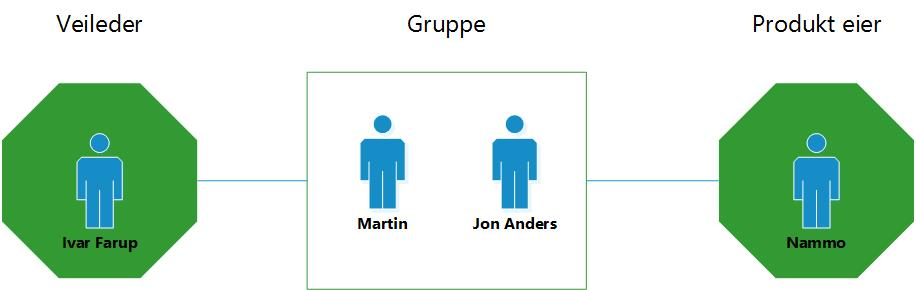
\includegraphics{Scrumroller1}

Figur 1 : Representasjon av scrum rollene


\section{Akademisk bakgrunn}
De siste 3 årene har begge medlemmene studert ved Norges teknisk-naturvitenskapelige universitet. Martin har studert programvareutvikling og Jon anders har studert Data ingeniør. Dette har gjort at vi begge har mye av den samme kunnskapen men i tillegg erfaringer i forskjellige felt. Dette har gitt oss en tyngde i forskjellige programmeringsspråk som C++, java, mysql, php, javascript og andre scriptspråk som bash og powershell. Martin har i tillegg tatt er ergonomi i digitale medier fag. Som fokuserer på brukerinteraksjon med systemet. Jon Anders har erfaring med matte 1 og 2, noe som ble brukt mye under utviklingsprosessen. Den største forskjellen mellom oss har vært mattekunnskapene, den har ført til at Jon Anders ble jobbende hovedsakelig med algoritmen og andre matematiske krevende arbeid. Martin ble jobbende mer med oppgaver som ikke krevde så mye matematiske ferdigheter, som GUI, design rapportskriving og andre funksjonaliteter som eksportering til Excel.



\section{Dokumentstruktur} 

\textbf{Introduksjon}\\
dette kapittelet presenterer prosjektet til leseren, introduserer gruppen, arbeidsgiveren og veilederen, samt generell informasjon om prosjektet\\

\textbf{Prosjektorganisering}\\
Dette kapittelet introduserer leseren til utviklingsprosessen og store avgjørelser som ble tatt tidlig i prosjektet.\\

\textbf{Kravspesifikasjoner}\\
	Dette prosjektet gir en dypere introduksjon til kravspesifikasjonene.\\

\textbf{Teknisk Design}\\
Dette kapittelet gir en oversikt over valget av språk, rammeverk, utviklingsmiljø, hvordan vi har tolket kravspesifikasjonene og arkitektur designet.\\	

\textbf{Implementasjon}\\
Dette kapittelet viser en oversikt over hvordan de viktigste funksjonene har blitt implementert.\\ 

\textbf{Utviklingsprosess}\\
Dette kapittelet gir leseren et innblikk i utviklingsprosessen , hvilke problemer vi har møtt og hvordan vi har valgt å løse dem.\\

\textbf{Testing og Kvalitetssikring}\\
	Dette kapittelet gir et detaljert innblikk i hvordan vi har testet og kvalitetssikret koden.\\

\textbf{Diskusjon}\\
Dette prosjektet inneholder en diskusjon av hele prosjektet, sammenlikning av oppgaven opp mot resultatet. Gruppen sin refleksjon av arbeidet som har blitt gjort og resultatet som har blitt levert.\\

\textbf{Konklusjon}\\
	Dette kapittelet konkluderer kort hele prosjektet og rapporten.\\





  
\chapter{Kravspesifikasjoner}



Dette kapittelet vil ta for seg kravene som blir satt for funksjonelle krav i tillegg til supplementære krav. Disse skal hjelpe med å forstå hva programvarens grunnleggende oppgaver og hva som kan legges til.

	Funksjonelle krav \\ \\
	kommer mer









\section{Use Case}
Denne delen vil vise funksjonalitet kravene til programvaren gjennom use case diagrammer. I det første diagrammet har vi en generell oversikt over funksjonalitetene til programvaren 


\begin{figure}[h]
    \centering
    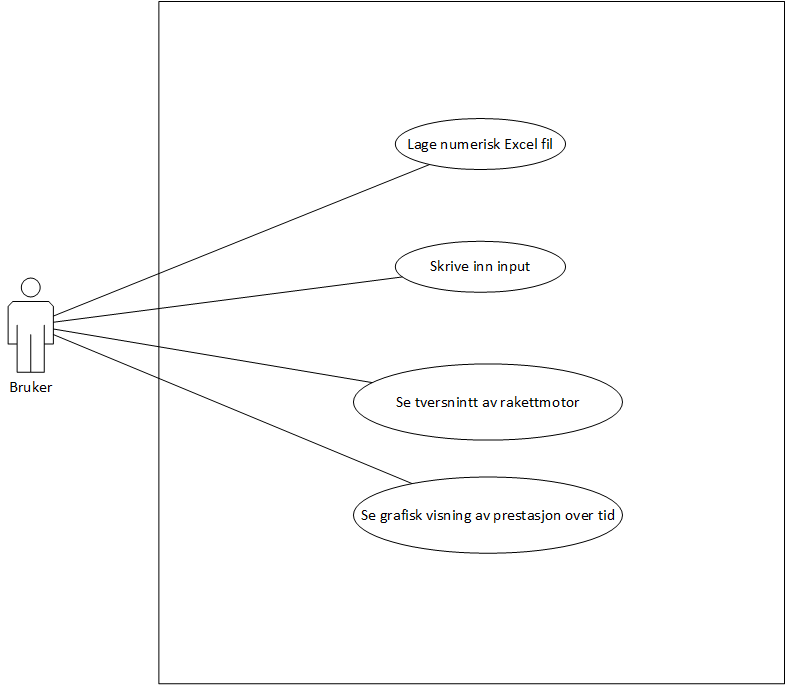
\includegraphics[width=\textwidth]{usecasepng}
    \caption{Use Case diagam}
    \label{fig:my_label}
\end{figure}

\section{Høynivå Use Case}
\begin{center}
  \begin{tabular}{ | l | p{8cm} | }
    \hline
    Use Case & Lage numerisk Excel fil \\ \hline
    Aktør & Bruker \\ \hline
    Hensikt & Lar brukeren eksportere data til en Excel fil\\ \hline
    Beskrivelse & Henter data om web, omkrets, portareal og webareal. Skaper Excel fil i filsystemt og legger hentet data inn i filen. \\
    \hline
  \end{tabular}
\end{center}

\begin{center}
  \begin{tabular}{ | l | p{8cm} | }
    \hline
    Use Case & Skrive inn input \\ \hline
    Aktør & Bruker \\ \hline
    Hensikt & Lar brukeren spesifisere parameter for modelleringen og beregningene\\ \hline
    Beskrivelse & Henter data fra brukeren og generer datamodeller og data basert på dette. \\
    \hline
  \end{tabular}
\end{center}

\begin{center}
  \begin{tabular}{ | l | p{8cm} | }
    \hline
    Use Case & Se tversnitt av rakettmotor \\ \hline
    Aktør & Bruker \\ \hline
    Hensikt & Viser datamodeller på skjermen\\ \hline
    Beskrivelse & Henter en ferdiggenerert datamodell som speiles og roteres før den vises. \\
    \hline
  \end{tabular}
\end{center}

\begin{center}
  \begin{tabular}{ | l | p{8cm} | }
    \hline
    Use Case & Se grafisk presentasjon over tid \\ \hline
    Aktør & Bruker \\ \hline
    Hensikt & Lar brukeren se hvordan brennoverflaten utvikler seg\\ \hline
    Beskrivelse & Viser en graf av omkrets over web (tid), basert på eksisterende beregninger. \\
    \hline
  \end{tabular}
\end{center}

\section{Design Krav}
Et av de meste etterspurte funksjonalitetene var en grafisk visning av hvordan rakettmotoren vil bli seendes ut. Denne visningen gir brukeren muligheten til å se hvor den initiale utskjæringen er, og hvor bred motoren er ved en visning av tankveggen. Mellom disse to blir brukeren vist hvordan den initiale utskjæringen vil forandre seg steg for steg. Avstanden mellom hvert steg har blitt definert av brukeren, sammen med den initiale utskjæringen. 


\subsection{2D Modell} 
Brukeren skal kunne bygge opp en komplett drivstofftank, med komplett brennstoffprofil, basert på forhåndsdefinerte segmenter med gitte parametere for modifisering. \\ \\
Segmentene med parametere er:
\begin{itemize}
    \item Ytre og indre radius på sylinderform
        \begin{itemize}
            \item Den ytre radiusen er der brennstoffet møter innsiden av tanken.
            \item Den indre radiusen er hvor brennstoffet møter brennkammeret.
        \end{itemize}
    \item Utformingen av stjerneform
        \begin{itemize}
            \item Hver arm er parallell og enden er avrundet.
            \item Brukeren kan endre på bredden og lengden på hver arm og antall armer.
            \item Vinkelen mellom hver arm er lik, så antallet armer og størrelsen på hver vil implisitt bestemme vinkelen.
        \end{itemize}
\end{itemize}



	



\subsection{Beregning}
En av de viktigste delene av programvaren er beregningen av forbrenningen i tanken, hvis denne er unøyaktig er programvaren nær verdiløs. Vi skal utvikle en algoritme for hvert segment brukeren kan legge inn i tanken.	\clearpage
\subsection{Presentasjon}
\begin{itemize}
    \item Numerisk output\\
    
    Nammo vil ha muligheten til å få resultatene levert i et numerisk Excel format, der de får effekten over tid presentert i en tabell. Dette skal kunne brukes som input til andre programmer, så det nøyaktige formatet må bestemmes etter nærmere samtaler med Nammo.\\
    \item Graf\\
    
    Når brukeren har laget sin versjon av brennstoffet skal resultatene vises i en graf umiddelbart. Grafen vil kun vises så lenge modellen er komplett, før dette og om brukeren fjerner et segment vil grafen ikke vises. Så lenge modellen er komplett skal alle endringer oppdatere grafen med en gang.
    
\end{itemize}

	\subsection{Valg av plattform}
Vi ønsket at programvaren skulle ha så få begrensninger som mulig, men programvaren er kun tilgjengelig på Windows maskiner. Nammo hadde planer om å kjøre programvaren på deres arbeidsmaskiner som alle kjører nyeste versjon av Windows. Vi valgte derfor å ikke gjøre programvaren kompatibel med flere plattformer. Dette ble nedprioritert fordi Nammo ikke hadde behov for kryssplattform funksjonalitet og vi prioriterte den grunnleggende funksjonaliteten.


\subsection{Brukervennlighet}
Brukervennlighet er noe vi har satt stor fokus på, det var viktig for oss å skape et produkt som ga brukeren en glede under bruk. Hvis programvaren er tungvint å bruke vil den ikke blir brukt, vi setter derfor brukervennlighet på samme nivå som funksjonalitet. Det er derfor viktig for oss definere hva brukervennlighet betyr, ettersom ordet i seg selv er litt vagt. Jacob Nilsen definerer brukervennlighet i sin artikkel for Nilsen Norman Group[1]. I denne artikkelen forteller han at brukervennlighet er definert av fem komponenter(Learnability, Efficiency, Memorability, Errors, Satisfaction). Vi har valgt å ta for oss fire av disse her ( Learnability, Efficiency, Errors, Satisfaction ). Learnability definerer hvor lett det er for brukeren å plukke opp programvaren å bruke den. Efficiency definer hvor effektiv bruker kan bli etter bruker han har lært seg programvaren. Errors definerer hva som skjer når brukeren gjør feil. Klarer programvaren å håndtere inputen eller vil den krasje. i tillegg hvor vanskelig det er for brukeren å rette opp feilene som har blitt gjort. Satisfaction definerer hvordan brukeren trives under interaksjonen av programvaren, er den tung å bruke eller blir brukeren sittende med en godt følelse. \\ \\
For å lage vår programvare så brukervennlig som mulig har vi valgt å gi brukeren med en enkel og minimal framside. Brukeren blir møtt med en framside som tar i mot parametrene som definerer raketten. Brukeren trenger kun å oppgi disse å trykke kjør. Dette gjør at det ikke er noen mer kompliserte verktøy som kan øke effektiviteten for mer erfaren brukere. Når brukeren har oppgitt sine parametere blir fremsiden oppdatert og resultatet blir vist. Hvis brukeren har gjort noe feil vil han ikke bli straffet for det. Bruker har fortsatt muligheten til å endre parametrene som ble oppgitt. Denne effektive å enkle løsningen føler vi vil gi brukeren en god opplevelse under bruken.



\subsection{Språkstøtte}
Nammo er et internasjonalt firma som opererer i land som Norge, Sverige, Finland, Spania, Tyskland, India og USA. Nammo har kontorer i 12 forskjellige land over hele verden. Det er derfor viktig å utvikle et produkt som kan brukes av alle land. Nammo produserer mesteparten av sine rakettmotorer på sine lokaler i Raufoss, Norge og noen på sine lokaler i USA. Vi kan ut fra denne informasjonen anta at programvaren kommer til å bli brukt for det meste i Norge. Det er en liten sansynlighet for at den kan bli brukt i USA eller utenlandske arbeidere på Raufoss kan bruke programvaren. Programvaren bruker derfor engelsk i tillegg til at all kode og kommentering er skrevet på engelsk, hvis Nammo ønsket å videreutvikle programmet.

\subsection{Sikkerhet}
Programvaren vi har utviklet har ikke noen form for brukerkontroll. Nammo hadde ingen behov for noe sikkerhetstiltak eller identifikasjon av bruker ettersom det ikke er noe sensitiv informasjon i bruke under programmet og er mer et verktøy. Siden programvaren blir installert på en maskin og ikke blir brukt over internett er det liten fare for brudd av sikkerhet.

\subsection{Dokumentasjon og testing}
Nammo viste en interesse for å videreutvikle programvaren etter vår bacheloroppgave. Vi har derfor tatt hensyn til deres ønsker og satt opp en oversiktlig arkitektur som deler kildekoden opp i tre forskjellige grupper( Model, View, Controller ). MVC er en kjent og mye brukt i bransjen i dag. Vi har valgt å ta den i bruk for sin simplisitet i tillegg til sin popularitet. Vi mener at denne modeller gir kildenkoden en strukturert arkitektur som gir nye utviklere en god forståelse av funksjonaliteten.

	\subsection{Ytelse}
Nammo skal kjøre programvaren på sine vanlige arbeid laptoper, disse har en begrenset prosesseringskraft. Funksjonaliteten Nammo ønsker er krevende å er en av våre største utfordringer. Vi må ta hensyn til disse maskinene og effektivisere den grunnleggende algoritmen så den er så lett at den kan kjøre på brukerens maskin uten å skape frustrasjoner og påvirke brukervennlighet.

\subsection{Lisenser}
\begin{description}

\item \textbf{Python}\\
Utgitt av Python Software Foundation, under PYTHON SOFTWARE FOUNDATION LICENSE VERSION 2\cite{Python}
\item \textbf{TkInter}\\
Utgitt under Python lisensen, mens Tcl og Tk bibliotekene som TkInter laster inn er utgitt under BSD lisensen\cite{TkInter}
\item \textbf{Matplotlib}\\
Utgitt av Matplotlib Development Team under License agreement for matplotlib 2.0.2\cite{Matplotlib}
\item \textbf{Numpy}\\
Utgitt av NumPy developers under NumPy license\cite{Numpy}
\end{description}
\chapter{Teknisk Design}
\label{chap:technical}


\section{Teknologi}
Hele prosjektet har blitt skrevet i Python, vi valgte å utvikle programvaren i Eclipse PyDev utvidelsen. TKinter ble brukt til utvikling av GUI, vi valgte Tkinter fordi det var oversiktlig og lett å ta i bruk. Vi bruker MatPlotLib til å presentere grafen i 2D versjonen. Vi valgte å bruke denne fordi den var kompatibel med Tkinter. Vi valgte å skrive koden i Python fordi det er et høynivåspråk som er utrolig effektivt. Det kan spesielt håndtere grafiske 2D og 3D visninger. \\ \\

\section{System Arkitektur}
Vi har valgt å ta i bruk MVC som står for Model View Controller. MVC er en arkitektur modell som deler programvaren opp i tre forskjellige grupper. Disse gruppene representere en del av programvaren og skal gi en flyt av informasjon. Modellen består av Model som håndterer informasjon og logistikk.  View er all visning av informasjon, dette kan være ting som bilder, video, tekst eller diagram. Controller håndtere all informasjon som brukeren gir til programvaren, som blir gjort om til kommandoer som Model kan bruke.[2]

\begin{figure}[h]
    \centering
    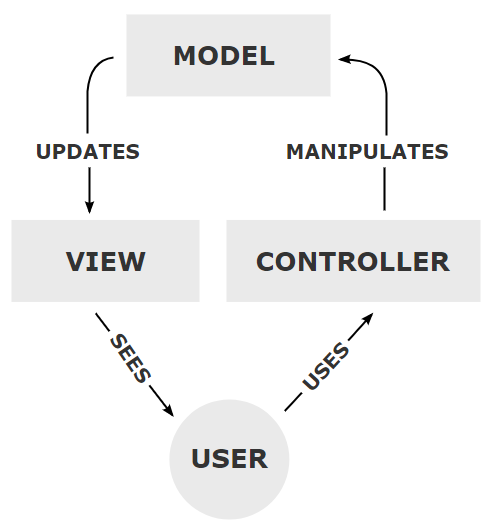
\includegraphics[width=8cm, height=8cm,]{MVC}
    \caption{Model View Controller diagram}
    \label{fig:my_label}
\end{figure}




\section{Arkitektur oversikt}
\subsection{Vår implementasjon av MVC}
I denne delen vil vi gi en oversikt over arkitekturmodellen vi har valgt å bruke. Nammo satte ikke noen krav til arkitekturen, de kom kun med en liste funksjonaliteter de ønsket oppfylt. Dette ga oss en stor frihet over hvordan vi kunne strukturere koden vår. Vi valgte å strukturere koden vår etter en MVC modell som har blitt kort forklart over. Vi valgte å bruke denne på grunn av dens vidsprede bruk i industrien, vår tidligere erfaring med arkitektur modellen og fordi oppgaven vår kunne naturlig deles etter MVC prinsippene. \\ \\
Arkitektur Modellen skal gjøre kildekoden oversiktlighet, som vil gjøre det lettere for nye utviklere å jobbe videre på programvaren etter dette prosjektet. Dette er vesentlig for programvaren fordi den er kun en tidlig utgave av det Nammo ønsker. Da det tidlig ble klart at vi ikke ville kunne implementere alle funksjonalitetene Nammo ønsket har vi hatt et stort fokus på å skape oversiktlig og velstrukturert kode. \\ \\
I Model delen har vi lagt inn dataobjektene, linjestykker og forhåndsdefinerte former som stjerner og tankveggen. De forhåndsdefinerte formene er satt sammen av linjestykker gitt vise parameter, og inneholder også data relatert logikk. Data relatert logikk sjekker at de gitte parameterene er innenfor gitte grenser, som at en stjernearm ikke er lengre enn radiusen til tankveggen.\\ \\
I View delen vil modellen og dataene etter simuleringen vises, og brukeren kan endre parameterene for modellen. Denne delen inneholder ikke noe logikk, da den kun mottar og viser data fra Controller delen og mottar og videresender data fra brukeren.\\ \\
I Controller delen skjer all applikasjonslogikken, som flytting av linjestykker etter som brennstoffet brenner opp og utregning av overflate og areal. Denne delen vil også mota brukerdata fra View delen og skape dataobjekter fra Model delen basert på disse dataene. De mest resursintensive delene av programmet skjer i denne delen da flyttingen av linjestykkene kan gi mange feil og derfor blir det her kjørt mange sjekker for å fjerne disse potensielle feilene.

\subsection{Klasse oversikt}
Klassen mover inneholder data om hvor langt hvert steg skal flytte linjestykkene, og hvor mange steg den har flyttet. Klassens viktigste funksjon er moveStep som flytter hvert linjestykke og kaller alle hjelpe funksjonene som sørger for at den nye formen etter flyttingen er riktig.\\ \\
Klassen lineSegment definerer et linjestykke med to endepunkt, og den beregner også lengden til linjestykket og den normaliserte normalen. Klassen innholder en del funksjoner for interaksjon med andre linjestykker, som å sjekke om to linjestykker er like, eller om de krysser hverandre.\\ \\
Klasser i shapes filen beskriver diverse former som blir brukt til skape stjerneformene og tankveggen i modelleringen. Vi her bare beskrive klasssen paraStar, da alle disse klassene er konseptuelt like og bare er ulike i hvilke former de skaper.\\ \\
Klassen paraStar skaper et dataobjekt med alle parameterene for å skape en halv stjernearm fra en stjerne med parallelle stjernearmer. Den inneholder funksjoner for å sette disse parameterene og en funksjon som generer den halve stjernearmen og returnerer en matrise med linjestykkene som beskriver figuren.\\ \\

\section{Språk og Rammeverk}

\subsection{Python}
Python er et høynivå språk utviklet på starten av 90 tallet. Python ble laget med filosofien som legger vekt på leselighet. Hovedsakelig ved bruk av mellomrom til å definere kode blokker i motsetning til semikolon og krøllparentes som blir brukt i mer tradisjonelle språk. Språket gir brukeren muligheten til å uttrykke begreper over få linjer kode i forhold til mer tradisjonelle språk som C++ eller Java. Pythons kompakte og effektive kode gjør det til et godt verktøy for utvikling av prototyper. Vi valgte å skrive programvaren vår i Python på grunn av språkets høynivå og mulighet til å presentere 3D modeller. Når vi undersøkt hvilket hvilket språk vi skulle ta i bruk ble Python anbefalt av veileder. Det var en positiv opplevelse å gå over til et høynivå språk, selv om mangel av semikolon og krøllparentes var uvant og bruke av mellomrom var litt av en overgang var vi fornøyde med valget. 

\subsection{Eclipce Pydev}
Når vi hadde funnet språket vi skulle utvikle programvaren i måtte vi velge et IDE. Vi valgte å bruke Eclipse med tredje part plug in Pydev. Eclipse er originalt brukt til utvikling av Java, men med dens enorm støtte fra tredjepart utviklere som tilbyr plug in, valgte vi å bruke Eclipse. Pydev er en av de mest brukte IDE for Python, Noe som ga oss en trygghet når vi møtte på problemer ettersom det var allerede noen som hadde møtt på det samme problemet før oss, og hadde funnet en løsning på problemet.


\subsection{MatPlotLib}
matPlotLib er et bibliotek utviklet for Python og den matematiske utvidelse NumPy. Den gir en objektorientert API som gir oss muligheten til å presentere en graf gjennom bruken av et GUI verktøy som Tkinter, qt, GTK+. MatPlotLib var lett å bruke sammen med Tkinter, vi bruke funksjonen pack() som satt opp grafen i Tkinter. Dette gjorde at vi raskt fikk opp funksjonaliteten, men design ble vanskelig. Ettersom vi brukte funksjonen pack() hadde vi lite kontroll over hvor den havnet. Vi prøvde å bruke en “grid” løsning, dette skapte kun problemer, og vi fikk ikke lengre vist grafen som vi ønsket.


\subsection{Tkinter}
Vi måtte ha en måte å presentere grafen vå på en brukervennlig måte som trakk brukeren til å bruke programvaren. Vi valgte å bruke Tkinter fordi den var kompatibel med MatPlotLib, i tillegg til at det var en lav læringskurve.
\chapter{Utviklingsprossesen}
\label{chap:process}


\section{Utviklingsmodell}
Oppdragsgiver uttrykte et ønske om tett oppfølging og innsikt underveis i prosjektet og god dokumentasjon for fremtidig vedlikeholdsarbeid. Det var også mulighet for endring eller tillegg av funksjoner i programvaren, så en smidig tilnærming var naturlig. \\ \\
På grunn av kravet til dokumentasjon tenkte vi raskt på Scrum som en god løsning og gruppen var allerede godt kjent med denne modellen. Vi undersøkte en del andre utviklingsmodeller, der Kanban og RUP kom frem som gode alternativ. Kanban er litt for løst strukturert for såpass uerfarne utviklere, siden det ikke er noen tidskrav for når hver funksjonalitet skal være ferdig. RUP er svært komplekst og ville ført til mye lengre planleggingstid om vi skal implementere den best mulig, siden vi ikke har noen erfaring med denne modellen.\\ \\ 
Under undersøkelsene kom vi over flere elementer fra andre utviklingsmodeller som ville være fordelaktige å implementere i vårt prosjekt. FDD har gode rutiner for å identifisere funksjonaliteter som legges til i backlogen\cite{FDD}. XP har mange gode verktøy for å standarisere koden og vi vil også implementere parprograming i størst mulig grad. Hvis en av oss ikke er i stand til å møte, eller et medlem jobber mer enn planlagt, vil vi gå gjennom endringene så fort vi har mulighet til å møtest. \\ \\
I implementasjonen vår av scrum vil Erland Ørbekk og Nils Kubberud fra Nammo ha rollen som Product Owners og Martin vil ha rollen som Scrum Master. Fordi vi ønsker å være selvorganiserende og lære mest mulig om estimering, vil Scrum Master ta på seg en del av ansvaret til Product Owners. Dersom Product Owners har noe spesifikt som de ønsker å prioritere vil det bli prioritert, men de har uttrykt et ønske om en mer veiledende enn bestemmende rolle i prosjektet. \\ \\
Vi valgte å ikke bruke alle elementene fra Scrum, vi valgte i stedet å bare plukke ut elementer som passet oss best. Elementer som daglige møter ble ikke holdt fordi vi hadde god kontroll over hva den andre jobbet med. Vi jobbet tett sammen som gjorde at vi hadde kontroll over hvor mye som hadde blitt gjort. Vi følte derfor at det ble veldig kunstig å ha et møte der vi diskutere progresjon, ettersom vi hadde full kontroll over motpartens arbeid.\\ \\
Vi brukte sprint elementene fra Scrum, vi satte opp møter med Nammo på slutten av hver sprint hvor vi forklarte hva som hadde blitt gjort denne sprinten. Vi klarte ikke å holde sprintene som vi hadde ønsket. Vi hadde problemer med feil estimering som gjorde at vi forandret sprintene. Vi jobbet videre med oppgavene vi hadde blitt utdelt, men oppgavene tok lengre tid enn estimert, det endte med at vi gikk bort fra sprinten.\\ \\
Vi brukte planing poker, men vi merket tidlig at vi fikk veldig lite fra tiden vi brukte. Vi klarte ikke estimere oppgavene,  og følte at hele prosessen var bortkastet tid vi heller skulle brukt på utvikling av programvare.\\ \\
Vi var veldig fornøyd med Srcum sin arbeidsmetode som jobbet på grunnleggende funksjonalitet som så bygges på videre, noe som er et kjerneelement i utviklingsmodellen.\\ \\


\section{Møter}

Møtene med Nammo valgte vi å sette opp litt etter vi hadde behov for dem, men vi prøvde å ta en tur til kontorene hver andre uke. dette ble satt opp litt etter behov, når vi hadde noen spørsmål som ikke lett kunne besvares på mail. Møtene ble i tillegg satt opp ettersom vi hadde noe å vise frem, en demo versjon for eksempel. Vi viste aldri Nammo noen direkt kode, men vi forklarte hva som hadde blitt gjort teoretisk så de kunne på bedre innsikt i hva som hadde blitt gjort. Det var lett å forklare teorien bak programmet ettersom Nils og Erland har en enorm mengde kunnskap i feltet sitt i tillegg gode kunnskaper i geometri og matematikk.\\
\\Et typisk møte på kontorene til Nammo på Raufoss, varierer på hvilket stadium i prosessen vi er. tidlig i prosessen brukte vi mye tid på hvilket verktøy vi skulle bruke, og hvilket som jobbet godt sammen. Når vi kommet lengre ut i utviklingsfasen, brukte vi møtene på spørsmål og uklarheter. Når vi hadde fått svar på det vi lurte på, forklarte vi hva som hadde blitt gjort og eventuelt vist en liten demo av hvordan ting virker. Dette ga Nammo en god oversikt over hvordan jobbingen gikk. Det var de fornøyd med og var mer interessert i noe som var gjort bygd fra bunnen så det kunne videreutvikles.

\subsection{Møte med veileder}
vi satt opp faste møter med Ivar hver tirsdag kl 13:00, disse møtene har hjulpet oss med å holde oss på rett spor. Møtene var avslappet og det var lett å komme med spørsmål og teorier. vi ble ofte sittende å tenke høyt på de største problemene. VI fikk mye ut av møtene, de var i tillegg lette å avlyse hvis det ikke var behov for dem eller det vare noe som krasjet. Etter å ha avlyst noen møter for bare å fortsette å jobbe når vi ikke hadde spørsmål. fant vi ut at det ikke var så lurt ettersom at vi hadde feiltolket oppgaven, merket vi at det er nyttig å ha møte bare for å passe på at vi holder oss på riktig spor.

\subsection{Gruppe møter} 
Vi avtalte å møte på skolen hver dag å jobbe, ettersom vi bare er to studenter på gruppen var det lett å møtes og jobbe sammen. vi jobbet tett i starten, med mye pairprogramming. Dette var nyttig, å jobbe sammen når vi begynte på et prosjekt som var ukjent for oss med et nytt programmeringsspråk. Når vi kom lengre ut i utviklingsprosessen ble vi jobbene mer hver for oss.


\section{Verktøy}
\subsection{Versjons kontroll}
Vi bestemte oss tidlig om hvilken versjonskontroll vi skulle bruke, det var egentilg ikke en avslutting men noe vi begge visste vi skulle bruke før vi begynte på prosjektet. Gjennom skolen gangen har vi brukt git siden andre semester. Når vi skulle ta for oss tema om versjonskontroll var vi begge enige om å bruke git. Git er den eneste versjonkontrollen noen av oss har brukt, så velge et nytt verktøy vi ikke har erfaring med virket ulogisk og tungvint. \\ \\
Vi valgte å hoste git repositoriet hos bitbucket, igjen fordi dette er det vi er vant til. Vi har såvidt prøvd github, men når vi satt opp repositoriet var det en vanesak å gå rett til bitbucket.
\subsection{Tekst editor}
Vi startet med å bruke Google docs som vår tekst editor. Vi valgte å jobbe på denne plattformen fordi vi ville ha en plattform vi kunne lett dele det som hadde blitt skrevet. Google Doc er i tillegg lett å ta i bruk det er ingen læringskurve i forhold til andre programmer som Latex. VI hadde originalt planlagt å bruke shareLatex som vår tekst editor. Vi hadde valgt å bruke denne løsningen fordi den ga oss muligheten til å dele dokumentet i tillegg til alle fordelene med Latex. Vi merket tidlig at en slik oppgave ikke passet i Google Docs, det var upraktisk og tregt å jobbe med store dokumenter i Google doc. Vi brukte da et dokument for hvert kapittel som var tungvint. Vi endte med å skrive de forskjellige kapitlene i hvert sitt Google Docs dokument for så å legge de inn i Latex. Vi valgte å gjøre det på denne måte fordi Latex gir et mye bedre slutt resultat enn Google Docs, men vi valgte å gjøre mesteparten av skrivingen i Google Docs fordi vi kunne lett skrive et utkast uten tanke på struktur. 

\subsection{IDE}
Når vi startet dette prosjektet viste vi ikke hvilken plattform vi skulle jobbe i. Det eneste vi hadde bestemt oss for var at vi skulle skrive programvaren i Python. Python var et språk ingen av oss hadde jobbet med før så vi hadde ingen preferanser. Vi endte opp med å bruke Eclipse sin utvidelse PyDev. Vi valgte å bruke denne plattformen fordi den var godt anbefalt i av Python miljøet i tillegg til at vi hadde begge en liten kjennskap til Eclipse. \\ \\
Vi trengte en måte å gjøre programvaren brukervennlig. Vi valgte derfor å ta i bruk Tkinter fordi det kom godt anbefalt i tillegg til at var kompatibelt med MatPlotLib. Vi så kort på qt som en mulighet for utvikling av GUI, men vi endte med Tkinter. Noe vi ikke var helt fornøyd med i ettertid på grunn av vanskeligheter til å plassere grafene på riktig plass. Vi fikk inn grafen fra MatPlotLib uten problemer, men etterhvert som vi implementert flere inputfelt og grafer  fikk vi ikke ting der vi ville. Vi valgte å bruke MatPlotLib for å viste brukeren hvordan stjerneformen han valgte ville bli seendes ut. 
\section{Problemer vi har møtt under utviklingsprosessen}


\subsection{Problemer med clicklistener og MVC}
Vi møtte tidlig på et problem med arkitektur modellen når vi skulle implementere visnings delen. Vi bruker her en clickListner() funksjon som konstant ser om en knapp har blitt trykket. Dette bruker vi vår brukeren oppgir parametere for rakettmotoren. I vår første prototype hadde vi ikke implementert en arkitekturmodell, vi kjøret hovedprogrammet for visnings filen. Når vi skulle implementere MVC møtte vi på en utfordring ettersom alle logiske beregninger skulle foregå i en annen mappe. Vi kunne ikke lengre bruke visnings modellen til å kjøre programmet å måtte finne en løsning på hvordan vi skulle kjøre programvaren. Løsningen vår var å lage en egen fil som kun håndtere overgangen mellom modellene. Denne inneholder syv funksjoner som gjør oppdaterer variablene og gjør det mulig for oss å bruke MVC.


\subsection{Minnekapasitet}
Et problem vi møtte på tidlig var størrelsen på arrayen vår. Med Nammo sitt krav på høy nøyaktighet måtte vi ha en enorm mengde punkter. Dette ville gi problemer i 2D, men spesielt for videre utvikling til 3D. I oppgaven vår skulle vi lage en solid 2D versjon som kan bygges videre på. Vi kunne se dette ville bli et problem når programvaren skal kjøres på en vanlig arbeids laptop.\\ \\
Vi tok problemet til veilederen der vi diskuterte problemet, etter en god stund kom vi frem til at hvis formen som skal skjæres ut er symmetrisk trenger vi ikke beregne hele formen, men i stedet bare en liten bit. Denne biten kunne da speiles, for en presentasjon. Vi kontaktet Nammo, som verifiserte at alle stjerneformede var symmetriske. Dette betyr at vi kan beregne en liten “kakebit” som kutter minneforbruket enormt. Vi så her at vi kunne dele opp formen på hver arm av stjernen. Så vi deler en arm i to biter, dette gjør at jo flere armer stjernen har, jo mindre er minneforbruket.



\subsection{Implisit vs Eksplisit}
Det største problemet vi møtte under denne oppgaven var desidert kollapsende vegger. Når en stjerneform brenner vil armene etterhvert krasje inn i hverandre og kollapse sammen. Dette skaper et stort problem for koden, fordi det er veldig vanskelig å vite om to punkter har krasjet eller om de holder på å kræsje. Vi har satt opp algoritmen så vi har en array med en rekke punkter, vi har ingen kontroll hvor de er i forhold til hverandre. Dette er det største problemet med eksplisitt løsning. Vi kunne gå over til en implisitt løsning som ville løst dette problemet, men det betydde at vi måtte begynne helt på nytt. i tillegg kommer en implisitt med en hel rekke nye problemer. \\ \\
En implisitt løsning betyr at vi har en flate dekket med punkter som er satt til 0. Når brennflaten vokser forflytter den som over punktene og når den passerer et punkt, blir det satt til 1. ( trenger bilde som forklarer ) Det største problemet med denne er minneforbruket. Det hadde vært en god løsning hvis nøyaktighet hadde vært så viktig. Med Nammo sitt høye krav på nøyaktighet ville dette gi store problemer. Vi måtte bruke en enorm mengde punkter for at algoritmen skulle bli nøyaktig nok. Vi valgte derfor å holde oss til en eksplisitt løsning.\\ \\
Måten vi valgte å løse dette problemet på var ved å bruke løsningen på minneforbruket. når vi delte opp formen laget vi en symmetrilinje. Vi vet at formen er symmetrisk dette gjør at vi kan håndtere de kollapsede veggene. Før hadde vi ikke kontroll over hvilke punkter som krysset hverandre. Dette gjorde at vi ikke ville klare å håndtere når veggene kollapset sammen. Når vi tar og deler stjerne armen på langs vet vi at den er identisk på den andre siden.\\ \\



\begin{figure}[h]
    \centering
    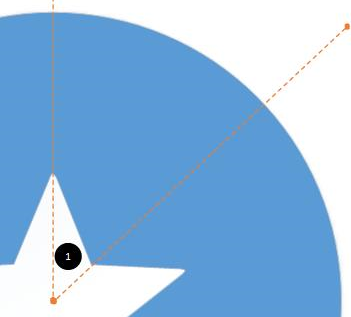
\includegraphics[width=\textwidth]{pngstjerne}
    \caption{Ilustrasjon av symemetrilinjen}
    \label{fig:my_label}
\end{figure}



\subsection{Symmetrilinjen}
kanskje skrive mer \\ \\
\clearpage

\subsection{Punkt forflytting vs linje forflytting} 
Vi møtte på et uforventet problem med forflytningen når vi begynte å nærme oss en ferdig prototype. Vi merket et problem rundt indre hjørner, et indrehjørne et hjørne som forflytter seg innover og holder sin vinkel, i motsetning til et ytrehjørne som vokser utover og får en mindre vinkel for hvert steg. \\
\begin{figure}[h]
    \centering
    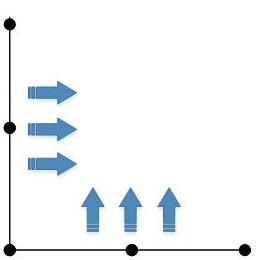
\includegraphics[width=0.5\textwidth]{nyindre}
    \caption{Ilustrasjon av indre hjørne}
    \label{fig:my_label}
\end{figure}

\noindent
Vi merket at det indre hjørnet ikke beholde vinkelen sin som den skal. Med vår punktvis forflytning, flytter alle punkter seg like langt. Dette skaper problemer i et indre hjørne, i et indre hjørne skal hjørne punktet flytte seg lengre enn de andre punktene for å beholde vinkelen sin. Med vår punktvis forflytning endte det med at hjørne punktet ble hengende igjen å lage en skarpere vinkel for hvert steg. For å løse dette problemet måtte vi endre den grunnleggende algoritmen i forflytningen.\\ 
\begin{figure}[h]
    \centering
    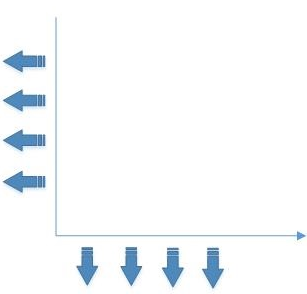
\includegraphics[width=0.5\textwidth]{nyytre}
    \caption{Ilustrasjon av ytre hjørne}
    \label{fig:my_label}
\end{figure}
\clearpage
\noindent
Vi valgte å løse dette problemet med å skrive om den punktvise forflytningen til en versjon som flyttet linjestykkene i stedet for punktene. Som vist øverst til venstre på figur \ref{fig:sloyfe} flytter vi hele linjestykket i stedet for punktene. Dette løser problemet med indre hjørner. Vi flytter hele linjen og når de krysser hverandre kan vi finne krysningspunktet på linjene og legge det nye punktet der. Da vil det indre hjørnet beholde vinkelen sin for hvert steg. \\ \\
\begin{figure}[h]
    \centering
    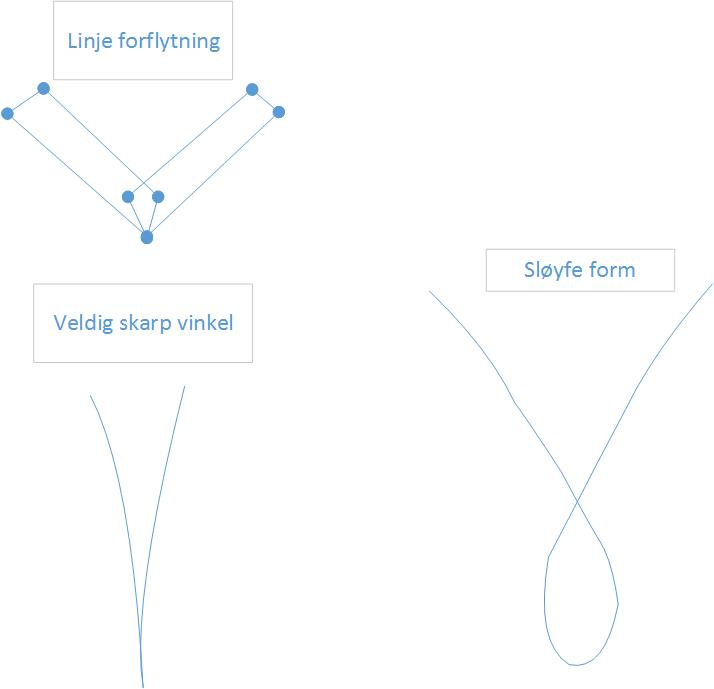
\includegraphics[width=0.5\textwidth]{pngSloyfeform}
    \caption{Ilustrasjon av linjeforflytning og sløyfeform}
    \label{fig:sloyfe}
\end{figure}

\noindent
Denne løsningen kom også med sine ulemper. Når et ytre hjørne forflytter seg minsker vinkelen dens, dette gjør at vi vil få tomrom mellom linjene våre. Så vi må legge på et lite linjestykke mellom hvert linjestykke i det ytre hjørne. Dette gjør at vi vil ha en eksponentiell økning av linjestykker i ytre hjørner. Vi måtte derfor modifisere algoritmen så den slår sammen linjestykker under en viss lengde for å minimere minneforbruket.\\ \\
Denne løsningen komme med flere potensielle problemer. Hvis algoritmen møter en veldig skarp vinkel kan linjestykkene flytte seg for langt. Dette gjør at algoritmen ikke oppdager at den har krysset sin nabo og vil fortsette å vokse å lage en slags sløyfe form. Dette er veldig usannsynlig hendelse, men vi valgte å ta hensyn til den for å gjøre algoritmen så robust som mulig.\\ \\
Måten vi løste dette på var ved å kjøre en for loop for hvert linjestykke i arrayen. Vi tar det linjestykke og sjekker om det krysser et annet linjestykke i arrayen. Hvis det krysser et annet linjestykke enn det ved siden av seg har det begynt på en sløyfeform.  

 






\chapter{Implementasjon}
\label{chap:implementation}
\section{Forflytting algoritme}
Vi hadde to forskjellige potensielle løsninger begge med sine fordeler og ulemper. Det første alternativet er eksplistitteflater. En eksplittflate er en flate med mange punkter forklar de forskjellige flatene
Implisitte flater gir oss høyest nøyaktighet prosent, men vi møter da på store problemer under forflytningen. vi har ingen måte og håndtere kollapsende vegger. Det er ikke noe problem i en sirkelformet 2D modell, men når vi må jobbe med forskjellige stjerneformer møter vi på et problem der veggen møtes og kollapser inn på hverandre. Når vi bruker implisitte flater må vi ha en løsning på hvordan vi skal kunne detektere når veggene møtes. Vi har ingen kontroll over hvor punktene ligger i forhold til hverandre vi har kun en liste med koordinater der punktene befinner seg og en liste med koordinater det punktene lyttes til. til slutt kommer det en utfordring med  minnebruk. Nammo krever en nøyaktighet prosent på 0.5 prosent alt over det er ubrukelig for dem. Vi kan begrense ressursene programmet trenger med å minske punktene, men dette kommer med sine ulemper. punktene er direkte knyttet til nøyaktighetprosenten, jo flere punkter jo høyere nøyaktighet prosent.\\ \\
Med disse problemene foran oss kom vi frem med en løsning der vi deler opp tverrsnittet til raketten. Alle raketten vi skal jobbe med er symmetriske, vi kan derfor dele den opp i mindre biter.Dette deler minnebruken med en enorm faktor, basert på antall armer. I tillegg til å gjøre programmet mer effektivt gir dette oss en løsning på vårt kollapsende vegger problem. Når vi deler opp tverrsnittet deler vi hver arm i to. Dette gjør at når armene treffer “symmetrilinjen” vil den kollapse med en annen arm. \\ \\
 Implisitte flater var veldig låvende til å starte med, vi kunne lett håndtere kollapsende flater, noe som var en stor utfordring med implisitteflater. Det største problemet med med denne metoder er nøyaktighet. Vi vil få problemer med å levere den nøyaktgheten Nammo krever. \\ \\
Etter å ha undersøkt og vurdert de forskjellige alternativene valgte vi å gå for eksplistteflater. Vi var ikke villige til å legge inn så store mengder arbeid til så ende opp med et produkt som ikke er nøyaktig nok. når vi kan dele opp raketten har vi en løsning på de største problemene, og er en sikrere avgjørelse mener vi. 
\clearpage 
Etter at vi valgte eksplisitteflater trengte vi å finne en løsning på hvordan vi skulle flytte den utover. vi startet med en liste med koordinater, dette er en liste med punkter som forteller oss hvor de befinner seg. vi måtte deretter flytte disse et steg utover. Vi startet da med å finne vektoren på linjestykke mellom punktene, vi tok så og fant normalen til disse linjestykkene. Med normalen til to linjestykker fant vi punktet midt mellom slutt punktet til normalen. Det er hit punktet skal flyttes, vi gjorde dette for hele listen. Vi kan bestemme hvor langt vi vil flytte linjen for hvert steg med å øke eller senke lengden på normalen. Det blir da laget en ny liste med punkter som inneholder punktet som ble funnet mellom de to normalene. Den liste med de gamle punktene blir da satt til den nye listen og så fortsetter prosessen videre til for løkken stopper.\\
\begin{figure}[h]
    \centering
    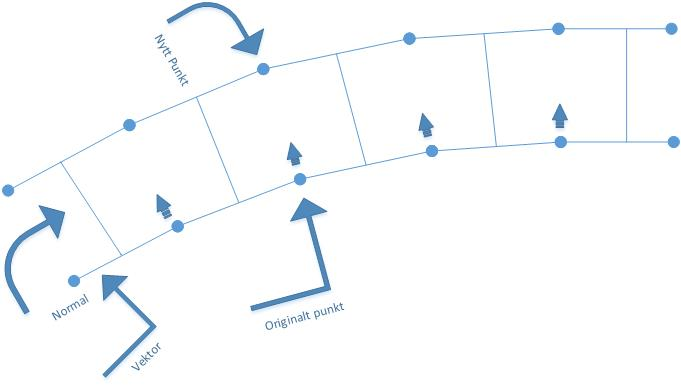
\includegraphics[width=\textwidth]{utviklingsmodell1}
    \caption{Ilustrasjon av punkt forflytting}
    \label{fig:my_label}
\end{figure}
Når vi klarte å flytte linjen konsistent over flere steg, la vi inn en yttre sirkel som skal illustrere tankveggen på raketten. Når linjen kommer hit er den tom for drivstoff og skal da stoppe. Vi la da inn en sjekk, som sjekker om linjen er innenfor denne sirkelen. Det siste steget blir ikke alltid et fullt steg, for hvis linjen møter på tankveggen skal linjen legge seg på tankveggen og ikke forflytte seg over denne. \\ \\
\begin{figure}[H]
    \centering
    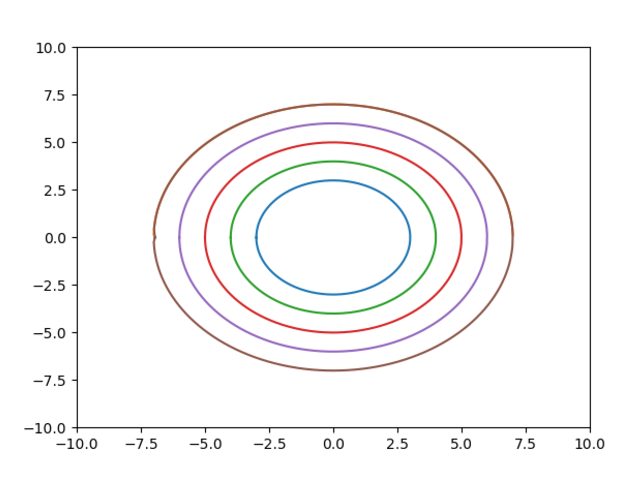
\includegraphics[width=\textwidth]{prototype}
    \caption{Ilustrasjon av tidlig prototype}
    \label{fig:my_label}
\end{figure}


\clearpage
\section{lineSegment}
Klassen lineSegment beskriver et linjestykke som består primært av to punkt som definerer endepunktene, lengden av linjestykket og den normaliserte normalen ut fra linjestykket. Ved flytting av endepunkter har vi utviklet en funksjon som rekalkulerer disse verdiene og oppdaterer de relevante variablene.
\begin{figure}[h]
    \centering
    \lstset{language=Python, breaklines=true,} 
    \begin{lstlisting}[frame=single]  
        def updatePoint(self, point, value):
            if (point == 'a'):
                self.a = value
            elif(point == 'b'):
                self.b = value
            else:
                stderr("Invalid input to updatePoint")
                return
            # compute normal
            self.dx = self.a[0] - self.b[0]
            self.dy = self.a[1] - self.b[1]
            self.magnitude = np.sqrt(pow(self.dx, 2) + pow(self.dy, 2))
            self.normal = [-self.dy, self.dx]
            # compute magnitude of normal
            self.normMagnitude = np.sqrt(pow(self.normal[0], 2) + pow(self.normal[1], 2))
            # normalize normal
            self.normal[0] = self.normal[0] / self.normMagnitude
            self.normal[1] = self.normal[1] / self.normMagnitude

\end{lstlisting}
    \caption{UpdatePoint funksjon}
    \label{fig:my_label}
\end{figure}


 Klassen inneholder også noen hjelpefunksjoner for å sjekke om to linjer er like, om to linjer krysser hverandre og om to linjer deler et punkt.
  \clearpage
 \section{Skape forskjellige former}
 Vi har en fil shapes som inneholder klasser for generering av de forskjellige formene, der tankveggen alltid blir generert og en av stjerneformene blir generert, basert på data gitt av brukeren. Ved å kalle getStarShape og getTankWall returnes en array av linjestykker som beskriver figuren, Star kan byttes ut med spesialiserte stjernetyper. 

\begin{figure}


 \lstset{language=Python, breaklines=true,} 
\begin{lstlisting}[frame=single]  
   def getStarShape(self):
        xs = []
        ys = []
        #rounding between each arm
        if (self.innerR > self.width):
            x1 = self.innerR * np.cos(self.theta / 2)
                #y = sqrt(r^2-x^2) => x = sqrt(r^2-y^2)
            x2 = nonClass.circle(-self.width, self.innerR)
            #from x1 to x2
            for x in np.arange(x1, x2, self.pointDistance):
                y = -nonClass.circle(x, self.innerR)
                if y <= -self.width:
                    ys.append(y)
                    xs.append(x)
        #draw straigth part of arm
        xs.append(x2)
        ys.append(-self.width)
        xs.append(self.length - self.width)
        ys.append(-self.width)
        #draw rounding of arm
        for x in np.arange(self.pointDistance, self.width, self.pointDistance):
            ys.append(-nonClass.circle(x, self.width))
            xs.append(x+self.length-self.width)
        # add last point     
        ys.append(0)
        xs.append(self.length)
        #returns the line segments for the points
        return nonClass.createLine(xs, ys)

\end{lstlisting}
    \caption{getStarShape funksjon}
    \label{fig:my_label}
\end{figure}
Stjernetypene er alle en sammensettning av rette linjer og delsirkler, der lengder, radier og avstander er gitt av dataen brukeren har tastet inn.

\clearpage
\section{Rotering}
Når en form skapes, er det bare en halv stjernearm som blir generert, og regnet på videre for å minimere beregningskostnader. \\
\begin{figure}[H]
    \centering
    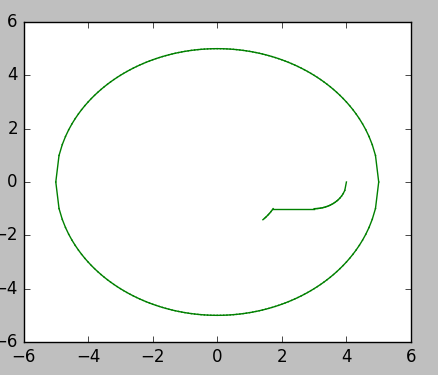
\includegraphics[width=\textwidth]{halfArm}
    \caption{Halv stjernearm}
    \label{fig:my_label}
\end{figure}



\noindent
Før tegning blir figuren speilet og rotert så mange ganger som stjernen har armer ved hjelp å gange hvert punkt med rotasjonsmatrisen.

\begin{figure}
    \lstset{language=Python, breaklines=true,} 
    \begin{lstlisting}[frame=single]  
        theta = np.pi / n
        matrix = [[np.cos(theta), -np.sin(theta)],
                      [np.sin(theta), np.cos(theta)]]
    
    \end{lstlisting}
    \caption{Caption}
    \label{fig:my_label}
\end{figure}

Vinkelen mellom hver arm er funnet ved å dele en hel sirkel, 2* pi, på antall armer,  n.  Her er n halvparten av armene, derfor ganger vi ikke pi med 2.
\begin{equation}
Vinkel = \frac{(2\pi)}{n}
\end{equation}

\begin{figure}[H]
    \centering
    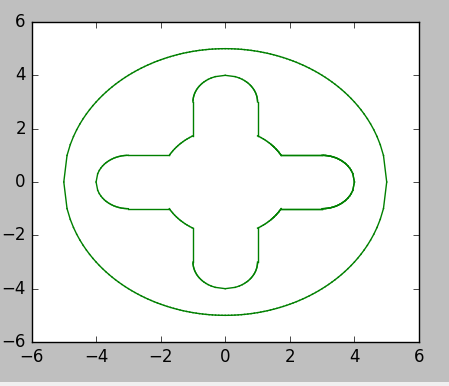
\includegraphics[width=\textwidth]{starShape}
    \caption{ferdig rotert stjerne}
    \label{fig:my_label}
\end{figure}


\section{Forflytting av linje}
Når et linjestykke skal forflyttes beregner bruker vi normalen til linjestykke ganget med forflyttingavstanden, som har blitt forklart i Utviklingsprosessen. Denne operasjonen skjer i funksjonen med navnet drawStep som ligger i filen moveLine. Denne funksjonen kjører en for løkke som går gjennom alle linjestykkene og flytter dem en etter en. De nye stykkene blir lagt i listen newSegment. På dette stadiet har vi to listen en som inneholder den originale linjestykkene og newSegments listen som inneholder linjestykkene som har blitt forflyttet. Denne funksjonen kjøres for hver forflytting, funksjonen avslutter med å sette newSegment til den gamle listen slik at newSegment kan igjen bli brukt til det neste steget i forflyttingen.
\clearpage
\begin{figure}
\lstset{language=Python, breaklines=true,} 
\begin{lstlisting}[frame=single]  
    def drawStep(self, shape):
        newSegments = []
        # move all segments
        for x in range(0, self.segments.__len__()):
            segment = self.segments[x]
            # move linesegment mveDist length along normal
            segment.moveSegment(self.stepSize)
            newSegments.append(segment)
        
        line = lineSegment.line(segment.b, [shape.length + self.stepSize*self.iteration, 0])
        newSegments.append(line)
        # check that all segments are connected and not ovelapping
        self.segments = nonClass.segmentOverlapControll(newSegments)
        self.segments = nonClass.segmentLengthControll(self.segments, shape.pointDistance * 2)
        self.segments = nonClass.symmetryLineControll(self.segments, shape.theta/2, shape.outerR) #Check symmetri line
        self.segments = nonClass.tankWallControll(self.segments, shape.outerR) #Check R vs outerR
        return self.segments

\end{lstlisting}
    \caption{DrawStep funksjon}
        \label{fig:my_label}
\end{figure}
Selve beregningen av hvor linjestykke skal bli plassert skjer i funksjonen moveSegment ligger i filen lineSegment. 
\begin{figure}
\lstset{language=Python, breaklines=true,} 
\begin{lstlisting}[frame=single]  
    def moveSegment(self, moveDist):
        
        moveX = self.normal[0] * moveDist
        moveY = self.normal[1] * moveDist
        self.a = [self.a[0] + moveX, self.a[1] + moveY]
        self.b = [self.b[0] + moveX, self.b[1] + moveY]
        

\end{lstlisting}
    \caption{moveSegment funksjon}
        \label{fig:my_label}
\end{figure}
\section{GUI}
Gui gir brukeren muligheten til å definere hvordan formen skal bli og hvordan den vil se ut. Her blir brukeren møtte med et enkelt brukergrensesnitt som gir han mulighetene til å definere seks forskjellige variabler.
\input{deployment}
\chapter{Testing og kvalitetssikring}
\label{chap:testing}


\section{Kode gjennomgang}
Vi hadde jevnlig kode gjennomgang der vi gikk gjennom det vi hadde jobbet på siden sist. Den som hadde skrevet koden forklarte de nye eller endrede funksjonene og den andre ga tilbakemelding på kodekvalitet, kommentering og valg av løsning. Disse gjennomgangene var uformelle og i etterkant burde vi ha hatt bedre retningslinjer for dette. Vi har refraktorert flere ganger i løpet av utviklingsprosessen og bedre kodegjennomgang kunne nok ha spart mye arbeid med dette. \\ \\

\section{Testing}
Vi har hatt en regel om at all kode som skal sendes inn til repositoriet skal være fungerende, men det har vært opp til hver utvikler å sørge for dette. Det hendte at denne regelen ble brutt, når når en utvikler skiftet arbeidsstasjon, men i disse tilfellene kom det godt fram at funksjonen ikke var ferdig, både i koden og i commiten. Vi har hatt to store feil i løpet av utviklingsprosessen, den ene var hvordan vi flyttet indre hjørner som beskrevet i “Problemer vi har møtt”, og den andre var en feil ved symmetrilinjene dersom det var flere enn fire armer på stjernen. \\
\begin{figure}[H]
    \centering
    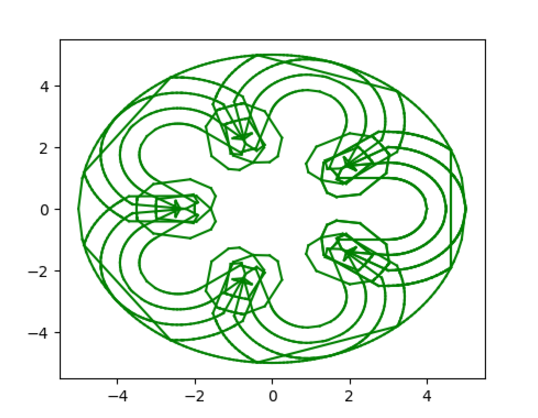
\includegraphics{testDemo}
    \caption{2D Modell med rotasjons feil}
    \label{fig:my_label}
\end{figure}
\noindent
Dette ble ikke plukket opp under testingen av funksjonen, men kom frem under senere testing.\\ \\
\noindent
Vi opplevde at testingen vår fungerte bra, da det bare var et vesentlig problem som ikke ble fanget opp. På tross av dette bør vi ha bedre retningslinjer for dette i fremtidige prosjekter, da vår fremgangsmåte er avhengig av at utviklerne er disiplinerte og lager gode tester på eget initiativ.\\ \\
\clearpage
\begin{figure}[h]

\lstset{language=Python, breaklines=true,} 
\begin{lstlisting}[frame=single]
def circleCrossing(line, r):
    p1 = line[0]
    p2 = line[1]
    #x^2*|p1|^2 + (x^2-2x+1)*|p2|^2 + 2x(1-x)*p1*p2 = R^2
    #(x^2-2x+1)*|p2|^2 = x^2*|p2|^2 - 2x*|p2|^2 + |p2|^2
    #2x(1-x)*p1*p2 = 2x*p1*p2 - 2x^2*p1*p2
    #x^2*p1^2 + x^2*p2^2 - 2x*p2^2 + p2^2 + 2x*p1*p2 - 2x^2*p1*p2 -R^2 = 0
    # = x^2*|p1|^2 + x^2*|p2|^2 - 2x^2*p1*p2 -2x*|p2|^2 + 2x*p1*p2 + |p2|^2 - R^2
    
    dotP1 = abs(p1[0]*p1[0] + p1[1]*p1[1])
    dotP2 = abs(p2[0]*p2[0] + p2[1]*p2[1])
    dotP1P2 = p1[0]*p2[0] + p1[1]*p2[1]
    #x^2*|p1|^2 + x^2*|p2|^2 - 2x^2*p1*p2
    a = dotP1 + dotP2 - 2*dotP1P2
    #-2x*|p2|^2 + 2x*p1*p2
    b = -2*dotP2 + 2*dotP1P2
    #|p2|^2 - R^2
    c = dotP2 - pow(r,2)
    
    #x = (-b+-sqrt(b^2-4ac) / 2a
    alpha1 = (-b + np.sqrt(pow(b,2)-4*a*c)) / (2*a)
    alpha2 = (-b - np.sqrt(pow(b,2)-4*a*c)) / (2*a)
    print "alpha1: ", alpha1
    print "alpha2: ", alpha2
    if -1 <= alpha1 <= 1:
        return alpha1
    else:
        return alpha2

a = [1,0]
b = [1,2]
line = [a, b]
x = circleCrossing(line, 2)
#x*p1 + (1-x)*p2
crossing = [x*a[0] + (1-x)*b[0],
            x*a[1] + (1-x)*b[1]]
print crossing
\end{lstlisting}
\caption{Test funksjon}
\end{figure}
\noindent
Isolert testing av funksjon for å finne kryssningen mellom en sirkel og et linjestykke, gitt linjestykket og radiusen til en sirkel sentrert i origo.

\chapter{Diskusjon}
\label{chap:discussion}

\section{Resultat}
Vi startet på et prosjekt med et klart mål Nammo, ønsket et verktøy som kunne hjelpe dem estimere brennsyklusen til en faststoffrakett.  Når vi startet prosjektet var det uklart hvor mye vi ville klare å få til. Vi endte opp med en 2D versjon som hadde en godt grunnleggende algoritme som klarte å håndtere indre og ytrehjørner. Vi ble eninge med Nammo å fokusere å den grunnleggende algoritmen å gjøre den så god som mulig. Ettersom tidligere forsøk på oppgaven hadde møtt på problemer når de skulle gå fra en 2D modell til en 3D modell. Nammo ønsket derfor at vi skulle komme opp med gode byggeklosser som kunne utvides senere. Vi ble fortalt tidlig at vi var ikke de første som hadde jobbet med dette prosjektet. Nammo hadde jobbet i noen år til å få dette prosjektet gjennomført, men uten suksess. Under planleggingsfasen hadde vi problemer med å legge en konkret plan over utviklingsfasen. Vi hadde ingen erfaring med grafisk presentasjon eller 3D programmering. Prosjektet utvikles i Python, et programmeringsspråk ingen av oss hadde brukt før. Dette ga oss en stor utfordring i begynnelsen, vi brukte derfor mye tid i starten av prosjektet til å undersøke å lære mer om plattformen, miljøet og fagfelte vi skulle jobbe med. Når vi ser tilbake på prosjektet kan vi se at det har gått mye tid til undersøkelse av ukjent språk og mindre effektivt arbeid på grunn av vår mangel på erfaring med platformen vi jobbet på.\\ \\
\noindent
Vi hadde opprinnelig fått en oppgave som ba om en fullstendig 3D modelleringsverktøy. Vi oppgavet at dette ble formye arbeid og endret oppgaven til et 2D modelleringsverktøy som var tilrettelaget til videreutvikling. Vi står nå igjen med en programvare som har en god algoritme for videreutvikling og overgangen til 3D modellering.
	
\section{Arbeidsfordeling}
Under hele prosjektet har vi jobbet godt sammen, men arbeidsfordelingen kunne vært bedre. Jon Anders hadde en god bakgrunn i matematikk som Martin manglet i sitt studie som programvareutvikler. Dette førte til noen vasker i starten av prosjektet ettersom dette er en matematisk tung oppgave. Vi valgte å løse dette problemet med parprogramming som virket bra, spesielt når vi jobbet på et helt nytt språk. Dette gjorde så vi begge lærte språket i samme tempo og endte opp på samme nivå. Martin sin mangel på matematisk bakgrunn kom fort frem å gjorde at Jon Anders fikk gjort mer av programmeringen enn Martin som måtte bruke mye tid på å forstå de matematiske prinsippene vi brukte. Dette førte til at Martin ikke var like effektiv å fikk gjort mindre av kodingen.

\section{Estimering}
Vi hadde estimert vi skulle bli ferdig i god tid, i tillegg hadde vi estimert tid for retting av feil og problemer. Den originale estimeringen endte med å være helt feil. Vi var ikke i nærheten av det vi hadde planlagt. Dette kom ikke som en overraskelse, vi forventet at vi ville bomme på estimeringen. Når vi startet bachelor oppgaven hadde vi aldri jobbet med et prosjekt på denne størrelsen og vi hadde kun noen få erfaringer med estimering på små prosjekter. Med vår uerfarenhet, og det å jobbe med et språk vi aldri hadde brukt før, var vi klar over at estimeringen ikke ville være riktig. Vi måtte etterjustere estimeringen ettersom vi kom lengre ut i prosjekt. I den originale estimeringen hadde vi håpet å ha ca en måned til kun rapportarbeid.

\section{Hva kunne gjort anderledes}
Når vi ser tilbake på hva som kunne blitt gjort annerledes er det noen ting vi ville endret. Det største hadde vært å satt opp en mer strukturert hverdag. Hadde vi laget over mindre perioder kunne vi ha strukturert ting bedre og kanskje vært mer effektive. Dagene våre hadde ikke en fast starttid og fast arbeidsplass. Dagene vår startet med en fast jakt etter en arbeidsplass der vi kunne jobbe i fred, og diskutere mellom hverandre. på grunn av mangel av grupperom og det at klassen ikke har en av satt klasserom eller arbeidsplass var det ikke lett å finne seg et sted å jobbe. konkurransen på grupperom er stor og en må være tidlig ute og bestille rom 2 uker frem i tid. Hadde vi vært flinkere på å finne en fast arbeidsplass med god plan over hva som måtte gjøres innen denne dagen og denne uken. Istedenfor å jobbe på en fast arbeidsplass med en strukturert plan, ble vi sittende å bare jobbe videre, vi visste hva vi måtte gjøre ettersom det er en oppgaven som består av få kompliserte oppgaver istedenfor et prosjekt som for eksempel utvikling av en app der det er mye forskjellige implantasjoner en på holde styr på.\\ \\
\subsection{Eksplisitte- og Implisitteflater}
Når vi startet oppgaven møtte vi tidlig på spørsmålet om vi skulle bygge programvaren med eksplisitte- eller implisitte flate. Vi valgte å bruke eksplisitt flate, fordi vi var redd for at en implisitt løsning ikke ville være nøyaktig nok. Vi valgte derfor å bruke eksplisitt flate som hadde større utfordringer og krevde mer arbeid, men hadde større sannsynlighet for mer nøyaktighet. Når vi ser tilbake på hvilke valg vi har tatt og hvordan vi har valgt å løse forskjellige problemer, er implisitt løsning det vi har vurdert mest. Med løsningen vi har når beregner vi en liten del av rakettmotoren, dette er en effektiv løsning som sparer minneforbruket. Hadde vi valgt en implisitt løsning hadde vi ikke møtt på problemet med kollapsende vegger å aldri tenkt på å beregne en liten bit av rakettmotoren. Når vi nå ser tilbake trur vi at en implisitt løsning kunne vært bedre. Noen av løsningene vi har brukt i vår versjon kan bli brukt i en implisitt løsning å senke minneforbruket til et nivå der vi kanskje kan oppnå nøyaktigheten vi trenger. Vi mener da at hadde vi visst det vi gjør nå hadde vi valgt en implisitt løsning som kun beregner en halv stjerne arm og speiler denne. Noen av de største problemene vi har møtt med en eksplisitt løsning er forflytting, detektere når brennstoffet har nådd tankveggen og symmetrilinjen. Disse problemene hadde vært mye mindre jobb og kunne vært mer effektiv.


\subsection{Valg av brukergrensesnitt}
Når vi undersøkte hvordan vi skulle lage brukergrensesnittet valgte vi Tkinter. Dette kom anbefalt fra Python miljøet, i tillegg til at tkinter er kompatibelt med MatPlotLib. Tidlig i utviklingsfasen var vi fornøyd med Tkinter, vi fikk lagt inn lagt inn grafen vi ønsket ved bruk av MatPlotLib. Vi møtte på noen små utfordringer, men fikk hoved funksjonaliteten til å virke som vi ønsket. Når vi senere skulle jobbe med design av brukergrensesnittet, møtte vi på store problemer. Vi hadde brukt en funksjon Tkinter har som heter Pack(). Denne dytter elementet inn på den første plassen som er ledig. Denne plasserte ikke grafen der vi ønsket den og når vi prøvde andre løsninger Tkinter tilbydde hadde vi ingen suksess. Den andre løsningen Tkinter tilbyr er en Grid() funksjon som deler vinduet opp i et grid og lar deg plassere elementene der du ønsker. Denne løsningen virker ikke med MatPlotLib vi hadde derfor elementer vi ikke kunne kontrollere. Vi oppdaget dette på et stadie der vi ikke hadde tid til å gå tilbake å endre på det. qt så ut som en løsning, men visste ikke om den var kompatibel med MatPlotLib. Med det vi vet i dag hadde vi sett på qt først for å se om vi kunne brukt MatPlotLib eller en annet bibliotek for å vise frem elementene våre.





\section{Vidreutvikling}
Det er helt klart rom for videreutvikling, vi ble ikke ferdig med oppgaven som vi ønsket. Vi fikk en fungerende 2D modell som hadde en god grunnleggende algoritme, men vi ble ikke ferdig med 3D modellen. 3D modellen var noe vi ønsket vi skulle bli ferdig med, men kom ikke så langt som vi ønsket. Det er her helt klart en utvidelse fra 2D til 3D. I tillegg til en utvidelse til 3D er det små justeringer for å fin pusse algoritmen til å kjøre mer effektivt. Det er noen deler av koden som kanskje er mer effektiv i et annet språk som C++. Det er da mulighet for å ta en funksjon som kan lages i C++, dette er noe som må utforskes videre. 
Etter vi innså at vi ikke ville bli ferdig med den originale oppgaven, Diskuterte vi hva de ville ende opp med når vi var ferdig. Nammo hadde tidligere forsøkt å løse denne oppgaven uten noe suksess. De ønsket derfor at vi skulle gjøre den grunnleggende algoritmen til å virke optimalt på 2D modellen. De hadde planer om å fortsette med prosjektet videre etter vi hadde levert bacheloroppgaven. Et av medlemmene på gruppe har allerede akseptert jobb fra Nammo med stilling for videreutvikling av prosjektet. 






\chapter{konklusjon}
\label{chap:conclusion}

Vi har nå kommet til et punkt hvor vi har fått muligheten til å jobbe med et spennende prosjekt som har vært krevende. Det har blitt lange dager og langer netter med mye jobbing som har vært lærerikt. Vi har gjennom denne oppgaven fått muligheten til å jobbe med et stort prosjekt lignende det vi vil møte i arbeidslivet. Denne oppgaven har gitt oss mange utfordringer som har utviklet våre ferdigheter som utviklere i IT bransjen. Vi fikk muligheten til å jobbe med Python, og programmering for brukergrensesnitt noe som var helt nytt for oss. Programmeringen for brukergrensesnittet har vært interessant og forfyllede. VI fikk for første gang jobbet med et prosjekt som virkelig tok form. Når vi hadde fått implementert brukergrensesnittet begynte vi se programmet ta form, det var ikke lengre et program som spyttet ut noen tall på en svart skjerm.\\
Vi har under dette prosjektet fått muligheten til å jobbe sammen som et profesjonelt lag over en lang periode som har gitt oss en uvurderlig erfaring. Selv om vi ikke fikk fullført oppgaven slik vi ønsket er vi stolte med det vi har levert.\\ \\
Når vi begynte på dette prosjektet satte vi oss noen mål som beskrev hva vi ønsket å lære under denne bachelor oppgaven. Vi har gjennom de siste månedene fått jobbet og lært oss Python. Vi har lært oss å levere et strukturert dokument skrevet i Latex, vi har fått en god innsikt i arbeid med 2D modellering med eksplisitte flater. I tillegg har vi fått et bedre innblikk i utviklingsmodellen Scrum i større prosjekter.


\bibliographystyle{ntnubachelorthesis}
\begin{thebibliography}{4}
\bibitem{Python}
    \emph{Python 2.7 license},
    \url{https://www.python.org/download/releases/2.7/license/},
    The Python Software Foundation,
    2017-01-12
\bibitem{TkInter}
    \emph{Tkinter Overview},
    \url{http://tkinter.unpythonic.net/wiki/Tkinter},
    AustinSavoy,
    2017-01-13
\bibitem{Matplotlib}
    \emph{License — Matplotlib 2.0.2 documentation},
    \url{https://matplotlib.org/users/license.html},
     Matplotlib development team,
     2017-01-13
\bibitem{Numpy}
    \emph{NumPy license — NumPy},
    \url{http://www.numpy.org/license.html},
    NumPy developers,
    2017-01-13
\bibitem{FDD}
    \emph{Feature-Driven Development (FDD)},
    \url{http://www.step-10.com/SoftwareProcess/FeatureDrivenDevelopment/index.html},
    Stephen R. Palmer,
    2017-01-17
\bibitem{Nammo}
    \emph{Nammo AS. About us [website]},
    \url{https://www.nammo.com/who-we-are/about-us/},
    Nammo AS,
    2017-01-23
\end{thebibliography}


\appendix %after this line all chapters will have leters instead of numbers
\chapter{Prosjektplan}


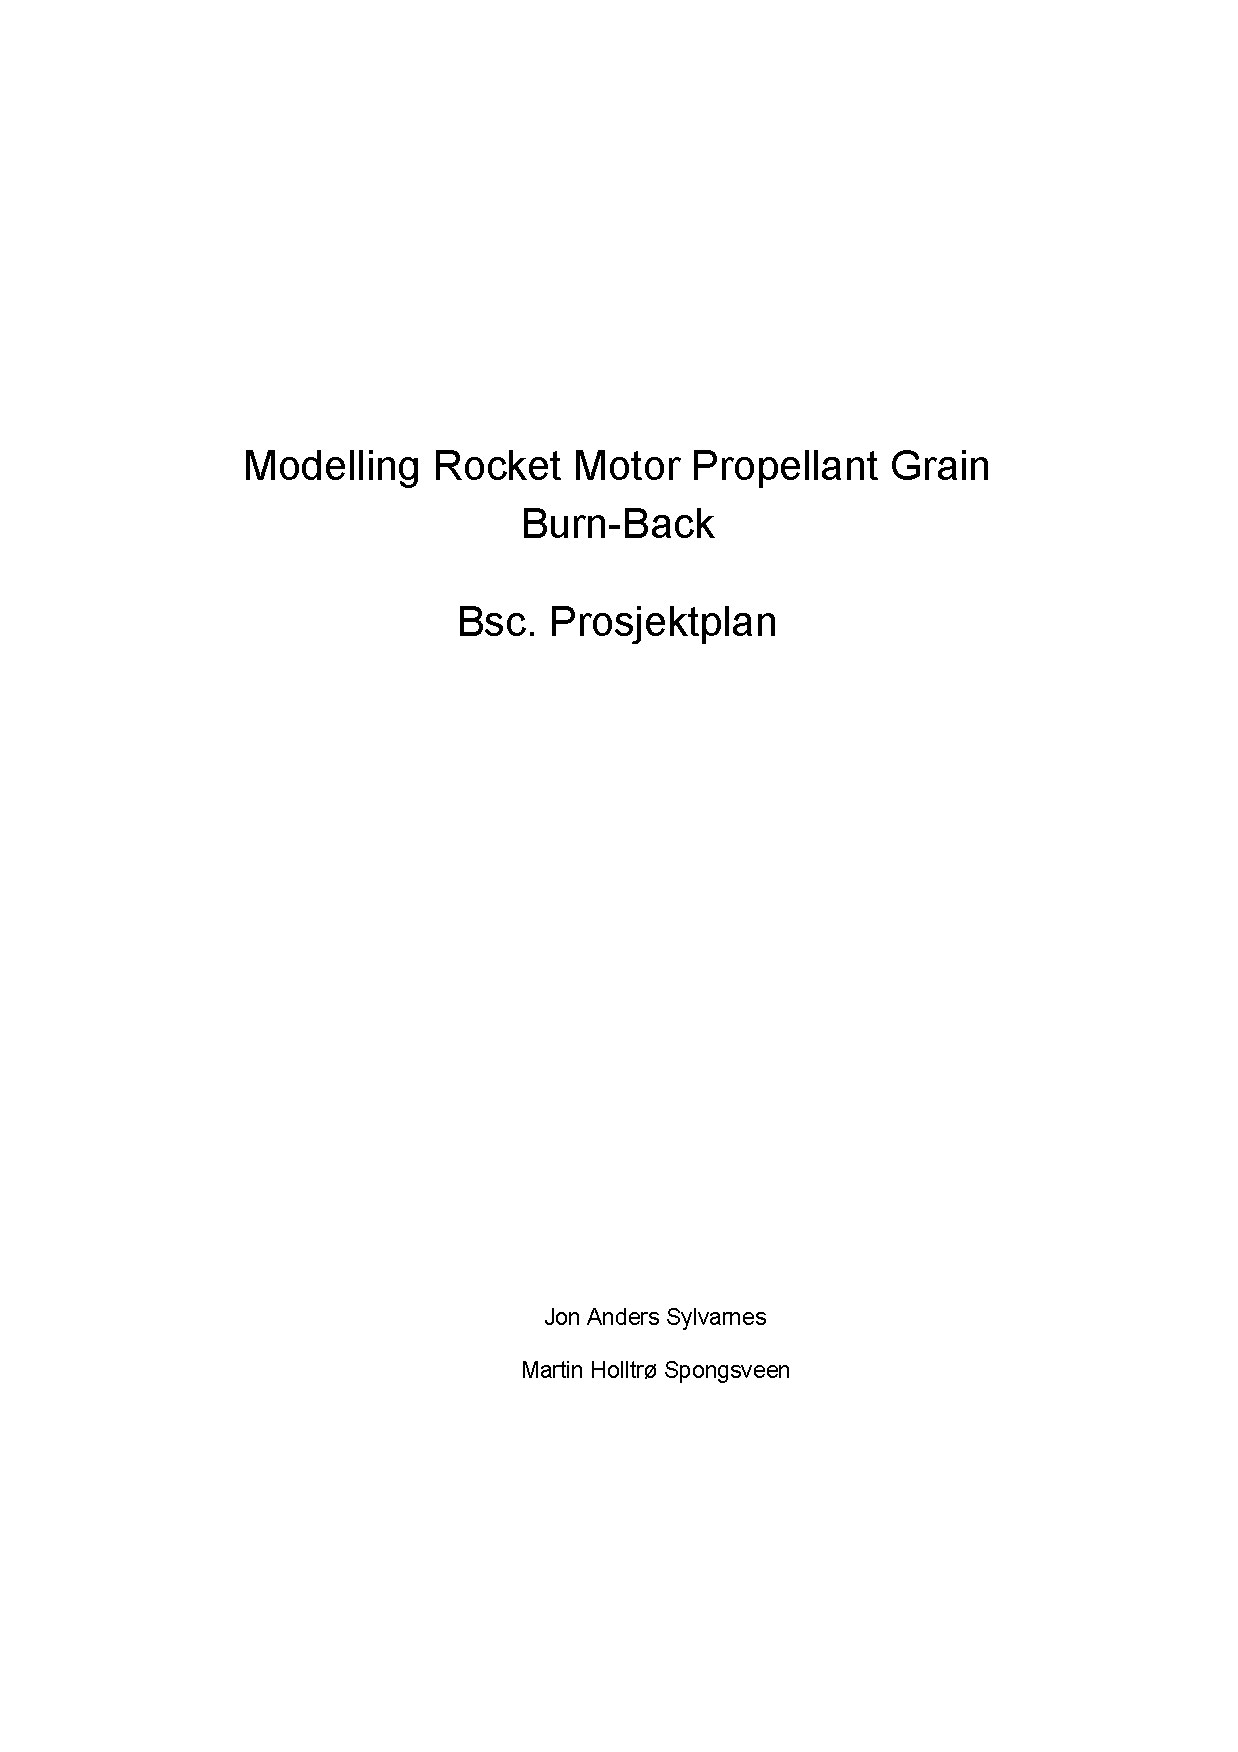
\includepdf[pages=-]{Prosjektstyring.pdf}

%\input{gantt}
\chapter{Møte Referat}

\section{Indroduksjonsmøte med Nammo - 13.01.2016}

\subsection*{Tilstede:}
\begin{multicols}{2}
\begin{itemize}
    \item Jon Anders Sylvarnes
    \item Martin Holltrø Spongsveen
    \item Nils Kubberud
\end{itemize}{}
\end{multicols}
\subsection*{\large Varihet: \enspace45 min}
\textbf{\Large Sammendrag}

\subsection*{Introduksjon}
Vi fikk en rask introduksjon inne fagfeltet, som ga oss den grunnleggene informasjonen vi trengte. Vi disukuterte oppgaven videre og kom til en god forståelse av hva de ønsket ut av programmvaren og hva vi mente var realistisk prosjekt.

\subsection*{Utviklingsprosess}
Vi spurte om Nammo hadde noe spessielle ønsker eller krav på hvordan vi skulle jobbe med prosjektet. Vi diskuterte emne og kom frem til at vi skulle velge prosessen som passet oss best. Kontakt personene ønsket hyppgie tilbakemeldiger, så vi valgte en smidig utvikligsprosess

\subsection*{NDA ( Non-disclosure agreement )}
Med høye sikkerhetsklareringer, spurte vi om det var behov for en NDA under dette prosjektet. Det var usikkert men tvilsomt.

\subsection*{Prosjektavtale}
Vi leverte Nammo med NTNU sin standard prosjektavtale. Den ble sendt videre sendt, og skulle bli underskrevet og sendt tilbake med e-post.

\subsection*{Versjonskontroll}
Vi diskuterte versjonskontroll, om Nammo hadde noen versjonskontroll de brukte lokat eller om vi kunne bruke Bitbucket

\subsection*{Videre møter}
Vi bestemte at vi skulle ha et møte på Raufoss to ganger i måneden, i tillegg til ukentlig status rapporter som blir sendt via e-post til oppdragsgiver og veileder.


\pagebreak

\section{Møte med Nammo - 06.02.2016}

\subsection*{Tilstede:}
\begin{multicols}{2}
\begin{itemize}
    \item Jon Anders Sylvarnes
    \item Martin Holltrø Spongsveen
    \item Nils Kubberud
\end{itemize}{}
\end{multicols}
\subsection*{\large Varihet: \enspace45 min}
\textbf{\Large Sammendrag}

\subsection*{Introduskjon}

Vi startet møte med Nammo med å fortelle hvordan arbeidet har gått så langt å hva vi jobber med. vi hadde en demonstrasjons av arbeidsmiljøet vi bruker og hvilket språk vi har valgt å bruke. vi viste et eksempel på en 3D modell, så de fikk et innblikk i hvordan et ferdig resultatet kunne bli. etter å ha diskutert de forskjellige utfordringene som står fremfor oss kom vi til en enighet at vi skulle ta et skritt tilbake. vi skal ta for oss det mest grunnleggende funksjonaliteten ettersom vi mener det er kritisk å ha en god algoritme i bunn vi kan bygge videre på. Nammo hadde tidligere jobbet med et prosjekt men hadde store problemer med algoritmen sin som slet med utvendige og innvendige hjørner. spesielt utvendige hjørner som kollapser 
%\input{progressreviews}
%\input{worklog}

\end{document}
